\documentclass[a4paper,11pt]{scrartcl}

\usepackage{graphicx}
\usepackage[utf8]{inputenc}
\usepackage{amsmath,amssymb,amsthm} 
\usepackage[round]{natbib}
\usepackage{url}
\usepackage{xspace}
\usepackage[left=20mm,top=20mm]{geometry}
\usepackage{algorithmic}
\usepackage{subcaption}
\usepackage{mathpazo}
\usepackage{booktabs}
\usepackage{hyperref}

\newcommand{\ie}{i.e.}
\newcommand{\eg}{e.g.}
\newcommand{\reffig}[1]{Figure~\ref{#1}}
\newcommand{\refsec}[1]{Section~\ref{#1}}

\setcapindent{1em} 

\renewcommand{\algorithmicrequire}{\textbf{Input:}}
\renewcommand{\algorithmicensure}{\textbf{Output:}}

\title{Zero-Shot Learning of Image Classification through Text-to-Image Generative Model}
\author{Fanyi Meng \\ \url{fanyimeng@link.cuhk.edu.cn}}
\date{March 22, 2024}

\begin{document}

\maketitle

\section{Introduction}
Zero-Shot Learning (ZSL) is a critical technique in machine learning,
enabling the recognition of unseen objects or categories beyond the scope of  training data. 
It excels in scenarios where comprehensive data collection is challenging.
This project proposes using generative models, like Stable Diffusion,
to fill data gaps by generating features of unseen categories.
The aim is to enhance ZSL's performance through experiments with these models,
thereby testing their ability to improve data richness and the ablity of generalizing  from known to unknown classes. 

\section{Related work}
\paragraph{Zero-Shot Learning} 
Zero-shot learning operates on the assumption that while no images of a new class are in the training set, 
other information like attributes or textual descriptions is available. 
Based on the connections between new class and training class in semantic space. 
The model can still classify these new class even corresponding data is not available. 
\citep{yu2010attribute}.Some work has already been done to integrate generative models with ZSL. \cite{mishra2018generative}
 trains a  Conditional Variational Autoencoder to understand the probability distribution
  of image features, thus improve the performance of ZSL. \cite{wang2018zero} used similar
   intuition and adapted the model for semi-supervised 
   and few-shot learning scenarios, 
   outperforming existing methods in tests on various benchmark datasets.







\paragraph{Text-to-Image Generative Model} 
Recently, with the advancement of large language models(LLM), 
there has been significant development in models capable of generating images from 
textual descriptions. 
This technology allows models to create visual content based on given text instructions.
Generative text-to-image models based on denoising diffusion probabilistic models
 \citep{ho2020denoising} such as Imagen \citep{saharia2022palette},
  Dalle-2 \citep{ramesh2022hierarchical}, and Stable Diffusion \citep{rombach2022high} 
can generate realistic high-resolution images and generalize to diverse text prompts. 
Their strong performance shows the feasibility of using generative models to provide data for new classes
\section{Research questions}

Following \citep{mishra2018generative}, our problem is described as follows: 
Given a set of train classes (seen classes) $\mathcal{Y}_{s}=\{y_{s}^{1},y_{s}^{2},...y_{s}^{n}\}$ and
a set of test classes (unseen classes) $\mathcal{Y}_{u}=\{y_{u}^{1},y_{u}^{2},...y_{u}^{m}\}$. 
For each class $y$ in $\mathcal{Y}=\mathcal{Y}_{u}\cup\mathcal{Y}_{s}$,
we have a class semantic embedding vector $A_{y}$, that $\textit{describes}$
the class. Given $d$-dimensional labelled training data from
the seen classes $\mathcal{Y}_{s}$ , i.e $\{X_{s},Y_{s}\}$. We will generate some new training data for the 
unseen classes $\mathcal{Y}_{u}$ based on the Text-to-Image Generative Model as mentioned in last part, and then we will construct a model $f\,:\,\mathbb{R}^{d}\rightarrow\mathcal{Y}_{s}\cup\mathcal{Y}_{u}$.
Finally we will test their performance and compare it with traditional zero-shot learning.
 
\section{Methodology}
We plan to utilize the same CNN architecture to perform three distinct tasks,
demonstrating the effectiveness of our approach across different scenarios:
Assume there are ten classes in the entire dataset, among which 8 classes are seen and two are unseen.
The first task involves training the CNN only on seen dataset.
And the model will be tested on the entire dataset. 
The second task involves training the CNN on the dataset which consists of seen data and generative data based on the label.
And the model will be tested on the entire dataset.
Based only on intuition,
the second task should achieve better classification 
performance since some additional features have been provided to the dataset. 
We aim to verify the extent of this performance improvement through specific experiments.
\begin{figure}[htbp]
  \centering
  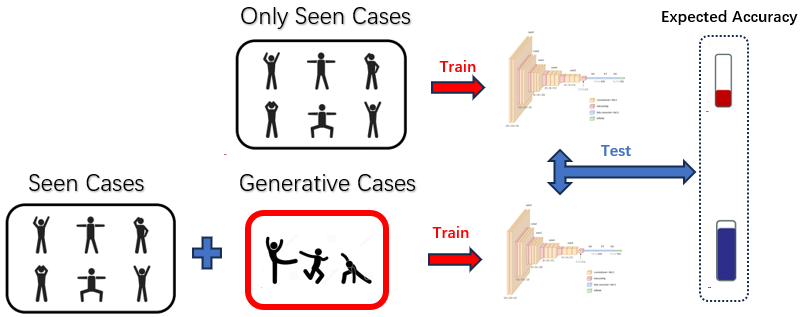
\includegraphics[width=1\textwidth]{pro.png}
  \caption{Workflow of Project}
  \label{fig:image1}
  \end{figure}

\section{Tools and datasets used}
We plan to use Dataset \cite{yang2023mm} to complete this work. This dataset contains datas of figures when human performing various actions. Additionally, it encompasses many other modalities of data like lidar.
If feasible, we consider extending this work to include these other modalities as well.

We plan to use \cite{chen2023llava} to generate new data, which combines three multimodal skills of pre-built AI models
without additional model training: visual chat of LLaVA , image segmentation
from SEEM , and image generation and editing from GLIGEN . So the generated data will be more closed to real data.
\bibliographystyle{abbrvnat}
\bibliography{myreferences}
\end{document}
